\chapter{Intro}\label{chap:intro}

\begin{figure}[!htb]
\centering
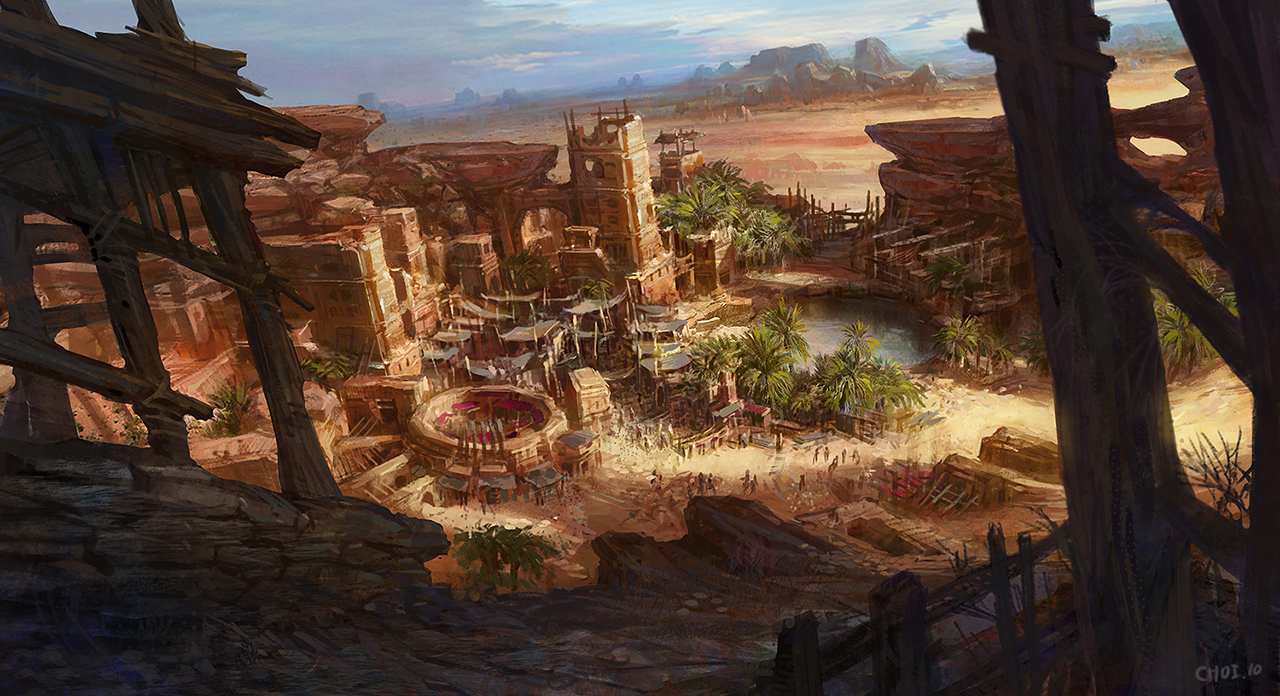
\includegraphics[width=0.8\linewidth]{images/city.jpg}
\end{figure}

\epigraph{\textit{
"For thousands of years, the Tablelands have remained untouched: its politics frozen in a delicate stalemate,
its life in a balance even more delicate. It is true that the Dragon Kings amused themselves with their petty
wars, rattling sabers to punctuate the passing of ages. It is true that, occasionally, another city would be
swallowed by the wastes.\\
\\
But there were no surprises. The Dragon Kings steered everything from their omnipotent perches, content in
their superiority, but ever thirsting for challenge. All that has changed. The Tablelands have been thrown into
turmoil, the likes of which have not been seen since times forgotten. The Dragon Kings have been thrown
into confusion, grasping for the tedium they so recently lamented.\\
\\
And yet I fear the worst is yet to come. Change is in the air, and change has never come gently to Athas."
} }{
Oronis, sorcerer‐king of Kurn
}

Athas' savage, primal landscape is the result of long centuries of ecological and magical abuses. The world is
dying. It breathes its last gasps as water turns to silt, grasslands become sandy wastes, and jungles decay into
stony barrens. Still, life finds ways to endure even in these hellish conditions. In fact, it thrives.
Children growing up beneath the crimson sun don’t aspire to become heroes. True heroes who champion causes
or try to make the world a better place are as rare as steel on Athas. Living to see the next dawn is more
important than defending a set of beliefs, so survival ultimately motivates all living creatures, not virtue or
righteousness.\\

Today, Athas rushes toward its future. If the course of destruction is to be diverted, if Athas is to be restored,
then heroes must grab the reins of destiny and give new hope and promise to the world. It will not be easy. In fact, it will
be extremely difficult. But it is possible. The denizens of the Tablelands have suffered under oppression for thousands of
years, and now, a boiling point has been reached. Perhaps not today, perhaps not tomorrow, but someday, change will
come.

\section{Eight Things You Need to Know}

The world of the Dark Sun setting is unique. This is not a world of shining knights and robed wizards,
of deep forests and holy shrines. Athas draws on different traditions of fantasy storytelling; simple
survival beneath the crimson sun is often its own adventure. With that in mind, here are the eight most
important things you need to know about the Dark Sun setting:

\begin{description}
    \item [The World is a Desert] Athas is a hot, arid world covered with vast
        stretches of desert—endless seas of dunes, stony wastes, thorny scrublands, and worse. In this
        forbidding world, cities and villages can only exist in a few oases or verdant plains. Beyond
        these islands of civilization is a barren wasteland roamed by nomads, raiders, and hungry monsters.

    \item [The World is Savage] Life is brutal and short in Athas. The vile institution of slavery is
        widespread in Athas, and hundreds, perhaps thousands, are sent to their deaths every year in
        bloody arena spectacles. Metal is quite scarce. Arms and armor are often made of bone, stone,
        wood, and other such materials, because steel is priceless.

    \item [Metal is Scarce] Most arms and armor are made of bone, stone, wood, and other such materials.
        Mail or plate armor exists only in the treasuries of Sorcerer-Kings. Steel blades are almost
        priceless, weapons that many heroes never see during their livetimes.

    \item [Arcane Magic Defiles the World] Athas was reduced to a wasteland by the reckless use of arcane
        magic in ancient wars. To cast an arcane spell, one must gather power from the living world around.
        Plants wither to black ash, crippling pain wracks animals and people, and the soil itself is
        sterilized; nothing can grow in that spot again.

    \item [Terrible Sorcerer-Kings Rule the Cities] The city- states of Athas are ruled by defilers of
        immense power. These mighty spellcasters have held their thrones for centuries. The sorcerer-kings
        govern through templars, a class of officials and lesser defilers who can call upon the kings’ powers.

    \item [The Gods of Athas are Silent] Athas is a world without gods. There are no clerics, no paladins,
        no real prophets or religious orders. In the absence of divine influence, people have turned to
        other sources of power. Psionic power is well known and widely practiced in Athas, while shamans
        and druids call upon the primal powers of the world - even though the primal spirits of Athas are
        often wild and vengeful.

    \item [Fierce and Deadly Monsters Populate the World] Athas is home to its own deadly ecology. Cattle,
        horses, camels— none of these animals can be found in Athas. Instead, people tend flocks of erdlus,
        ride on kanks or crodlus, and draw wagons with inixes and mekillots. Wild creatures such as lions,
        bears, or wolves are almost nonexistent. In their place are terrors such as the id beast, the
        so-ut, or the tembo.

    \item [Familiar Races aren't what you Expect] Many of the fantasy stereotypes don’t apply to Athasian
        heroes. On Athas, elves are a nomadic race of herders, raiders, peddlers, and thieves. Halflings
        aren't amiable river-folk; they're xenophobic headhunters and cannibals who hunt and kill anyone
        foolish enough to venture into their montane forests. Each of the major races has adapted to Athas
        in new and unexpected ways.
\end{description}
